\documentclass[11pt,a4paper]{article}

\usepackage[utf8]{inputenc}
\usepackage[T1]{fontenc}
\usepackage[margin=1in]{geometry}
\usepackage{amsmath,amssymb,amsfonts}
\usepackage{booktabs}
\usepackage{multirow}
\usepackage{tabularx}
\usepackage{hyperref}
\usepackage{url}
\usepackage{cite}
\usepackage{microtype}
\usepackage{graphicx}
\usepackage{upquote}
\usepackage{listings}
\usepackage{xcolor}
\usepackage{tikz}
\usetikzlibrary{positioning,arrows.meta,calc}

\hypersetup{
    colorlinks=true,
    linkcolor=blue!70!black,
    citecolor=green!50!black,
    urlcolor=blue!80!black
}

\lstset{
    basicstyle=\ttfamily\footnotesize,
    breaklines=true,
    columns=fullflexible,
    keepspaces=true,
    showstringspaces=false,
    showspaces=false,
    frame=single,
    backgroundcolor=\color{gray!10},
    keywordstyle=\color{blue!80!black}\bfseries,
    commentstyle=\color{gray!70!black}\itshape,
    stringstyle=\color{green!50!black}
}

\title{\textbf{The DOM Serialization Gap: Architectural Pruning, Information Loss, and Observation Confounds in Autonomous Browser Agents} \\[6pt]
{\large A Systems Audit and Case Study of browser-use 0.13.10}}

\author{
  Anonymous Authors \\
  \textit{Department of Computer Science} \\
  \texttt{Paper Under Double-Blind Peer Review}
}

\date{October 2026}

\begin{document}

\maketitle

\begin{abstract}
Autonomous web agents powered by Large Language Models (LLMs) are increasingly evaluated on multi-step transactional workflows. While existing benchmarks evaluate end-to-end task completion, the client-side Document Object Model (DOM) observation pipelines that prune and serialize web markup prior to model ingestion remain unexamined. In this paper, we conduct an empirical systems audit of the DOM serialization gap---the structural divergence between live browser representations and the serialized text ingested by LLMs---focusing on \texttt{browser-use 0.13.10} under text-only observation as a representative case study. Through static AST analysis and dynamic execution traces, we characterize three deterministic pruning bottlenecks that exclude structured Schema.org JSON-LD, strip non-interactive container WAI-ARIA labels, and omit custom developer \texttt{data-*} attributes. Comparing the agent's selector map against native Chromium DevTools accessibility trees, we document that 27 of 34 interactive elements ($79.4\%$) match Blink accessibility nodes on the tested route. Furthermore, we identify the Action-Label Co-Location Confound, an exploratory cloud pilot ceiling effect, and analytical sample-size boundaries demonstrating that small-sample evaluations ($n \le 20$ per arm) lack statistical power ($10.8\%$) to detect small effects ($\Delta = 0.20$), rising to only $49.6\%$ for moderate effects ($\Delta = 0.35$).
\end{abstract}

\textbf{Keywords:} Autonomous Web Agents, Large Language Models, DOM Serialization Gap, WAI-ARIA, Semantic Markup, Accessibility Trees, Experimental Reproducibility.

\section{Introduction and Research Motivation}
\label{sec:intro}

The integration of Large Language Models (LLMs) with automated browser execution environments has catalyzed the emergence of autonomous web agents capable of executing multi-turn transactional workflows across digital interfaces~\cite{zhou2024webarena, deng2023mind2web, drouin2024workarena, workarenapp2024, osworld2024}. Operating as sequential decision-making systems, these agents observe web page state, synthesize an action plan, and dispatch discrete interactions (e.g., clicking elements, typing text, selecting options) via browser automation protocols such as Playwright, Puppeteer, or the Chrome DevTools Protocol (CDP).

Despite widespread empirical benchmarking, contemporary web agent research suffers from a pervasive methodological confound: evaluations are typically conducted holistically across diverse web environments where visual styling, page layout, JavaScript routing logic, and DOM markup representations vary simultaneously. On complex websites, it is difficult to disentangle whether an agent failed due to visual occlusion, context saturation, stochastic planning drift, or uninformative DOM node labeling.

In modern frontend web engineering, information is intentionally partitioned into distinct architectural layers:
\begin{itemize}
    \item \textbf{Rendered Visible Typography:} Plain textual nodes rendered inside standard HTML tags (e.g., \texttt{<h1>}, \texttt{<p>}, \texttt{<span>}) intended for human visual reading.
    \item \textbf{Semantic Accessibility Markup (WAI-ARIA):} Programmatic semantic annotations (e.g., \texttt{role}, \texttt{aria-label}, \texttt{aria-describedby}) standardized by the World Wide Web Consortium~\cite{wai_aria12, accname11} to convey interactive semantics to assistive technologies.
    \item \textbf{Developer Custom Data Attributes:} Structured key-value pairs (e.g., \texttt{data-action}, \texttt{data-product-id}, \texttt{data-category}) utilized by client-side Single Page Applications (SPAs) for internal state management.
    \item \textbf{Structured Metadata (Schema.org JSON-LD):} Standardized machine-readable entity graphs embedded inside non-rendered script tags (\texttt{<script type="application/ld+json">}) for search engine indexing~\cite{schemaorg}.
\end{itemize}

As industry discussions propose modifying web architectures for autonomous agents---including proposals to enrich ARIA labels specifically for AI scrapers or to deploy dedicated machine endpoints (e.g., \texttt{llms.txt}~\cite{llmstxt2024}, Model Context Protocol APIs~\cite{mcp2024})---a fundamental systems question arises:
\begin{quote}
\textit{What information does a browser-agent observation pipeline preserve or discard between webpage markup, browser representations, and the final model observation?}
\end{quote}

If an agent framework silently purges structured metadata, web authors' efforts to markup pages for AI agents are lost. Furthermore, if researchers benchmark agent performance across markup variants without verifying prompt delivery, they risk evaluating an unaugmented text baseline while mistakenly attributing performance variations to invisible channels. 

In this paper, we address this question through an in-depth empirical systems audit of \texttt{browser-use 0.13.10} under text-only observation (\texttt{use\_vision=False}). We treat \texttt{browser-use 0.13.10} as a focused single-framework case study. Our contributions are strictly scoped to what our verified evidence establishes:
\begin{enumerate}
    \item \textbf{Source-Level Characterization:} We identify three deterministic pruning heuristics in \texttt{browser-use 0.13.10} that control metadata filtering and serialization.
    \item \textbf{Reproducible Reachability Tracing:} We trace information retention across five distinct pipeline representations, demonstrating that Schema.org JSON-LD and container ARIA attributes are excluded from the final observation stream under default configurations.
    \item \textbf{Comparative Accessibility Audit:} We compare the agent's interactive selector map against Chromium's native accessibility tree, reporting a 27/34 ($79.4\%$) correspondence census on the tested store route and characterizing the structural divergence between native accessibility caches and heuristic DOM serializers.
    \item \textbf{Experimental Confound and Power Analysis:} We formalize the Action-Label Co-Location Confound, disclose ceiling effects in an exploratory 41-trial cloud pilot, and calculate the sample-size boundaries required for valid equivalence testing in future web agent ablation benchmarks.
\end{enumerate}

\section{Related Work and Systems Framing}
\label{sec:related}

\subsection{Autonomous Web Agent Benchmarks}
Evaluation of LLMs as autonomous web agents has advanced through several benchmark suites:
\begin{itemize}
    \item \textbf{WebArena}~\cite{zhou2024webarena} established an end-to-end evaluation paradigm across four realistic self-hosted web applications, revealing task completion rates between $10.6\%$ and $14.4\%$. However, WebArena evaluates holistic task success across multi-page workflows, conflating layout design, visual rendering, and markup structure.
    \item \textbf{Mind2Web}~\cite{deng2023mind2web} introduced a dataset of 2,350 tasks across 137 real websites, evaluating element-level action prediction offline from DOM tree snapshots and demonstrating the severity of the raw HTML context bottleneck.
    \item \textbf{WorkArena and BrowserGym}~\cite{drouin2024workarena, workarenapp2024} evaluated web agents on enterprise workflows within ServiceNow. To mitigate context window exhaustion, BrowserGym utilizes Accessibility Trees (AXTrees), condensing long raw HTML documents into compact interactive token sequences. BrowserGym treats accessibility trees as an operational engineering optimization.
    \item \textbf{OSWorld}~\cite{osworld2024} extended multimodal agent evaluation to open-domain operating system tasks across heterogeneous applications, illustrating that execution grounding bottlenecks persist across diverse interface modalities.
    \item \textbf{WebAgent}~\cite{gur2024webagent} addressed HTML length bottlenecks by pre-training a specialized model to sub-sample and filter long documents prior to action planning.
    \item \textbf{AgentBench}~\cite{liu2024agentbench} evaluated LLMs across eight interactive environments, confirming substantial performance drops on web tasks relative to static reasoning benchmarks.
\end{itemize}

\subsection{DOM Observation Pruning and Distillation}
A critical challenge in web agent engineering is observation-space reduction:
\begin{itemize}
    \item \textbf{AgentOccam}~\cite{agentoccam2025} demonstrated that aggressive observation-space pruning yields a strong baseline for web agents, showing that reducing DOM size mitigates context bloat. However, AgentOccam focused on operational token reduction rather than auditing whether heuristic pruning selectively purges semantic metadata channels.
    \item Heuristic tag and attribute whitelisting in frameworks such as \texttt{browser-use 0.13.10} attempts to remove non-essential markup while preserving clickable elements. However, the precise information-loss characteristics of these heuristics have not previously been decomposed across frontend metadata channels.
\end{itemize}

\subsection{Multimodal Visual Grounding vs. Text Observation}
A parallel research line integrates computer vision with web navigation:
\begin{itemize}
    \item \textbf{VisualWebArena}~\cite{koh2024visualwebarena} extended WebArena to visually intensive tasks, showing that text-only agents fail when critical information is encoded exclusively in pixels.
    \item \textbf{SeeAct}~\cite{zheng2024seeact} formulated a two-stage visual agent framework separating candidate generation on screenshots from action grounding on DOM elements.
    \item \textbf{WebVoyager}~\cite{he2024webvoyager} evaluated multimodal agents using Set-of-Mark visual prompts across 15 live websites, achieving $55.7\%$ completion. Visual screenshot prompts bypass DOM observation pipelines entirely, trading structured machine semantics for pixel rendering.
\end{itemize}

\subsection{The Systems Audit Contribution}
Existing literature addresses task complexity, visual grounding, and model capabilities. However, prior studies have not systematically audited the client-side DOM serialization algorithms in open-source agent libraries to measure what information is preserved or discarded between source HTML, live DOM trees, browser accessibility trees, and final LLM prompt buffers. While auxiliary channels (such as page titles, current URL, active JavaScript execution tools, or visual screenshots) may supply additional context, the text-based DOM observation buffer remains the primary grounding mechanism for text-based browser agents.

\section{Systems Architecture and Pruning Heuristics in \texttt{browser-use 0.13.10}}
\label{sec:architecture}

We performed a static AST source-code audit and runtime execution trace of \texttt{browser-use 0.13.10} (PyPI binary release wheel distribution). The framework processes live web pages by walking the Chromium DOM tree and serializing it into a text string for the language model. We identified three deterministic pruning mechanisms:

\subsection{Script and Meta Pruning (\texttt{DISABLED\_ELEMENTS})}
In \texttt{browser\_use/dom/serializer/serializer.py} (Line 18), the framework defines an explicit exclusion set:
\begin{lstlisting}[language=Python]
DISABLED_ELEMENTS = {'style', 'script', 'head', 'meta', 'link', 'title'}
\end{lstlisting}
During simplified tree creation (\texttt{\_create\_simplified\_tree}, Lines 480--482):
\begin{lstlisting}[language=Python]
elif node.node_type == NodeType.ELEMENT_NODE:
    if node.node_name.lower() in DISABLED_ELEMENTS:
        return None
\end{lstlisting}
Any element matching \texttt{DISABLED\_ELEMENTS} is immediately pruned from the observation graph; child nodes are never traversed. Consequently, \texttt{<script type="application/ld+json">} structured data and \texttt{<meta>} tags are completely excluded from the serialized observation tree under this serialization path.

\subsection{Non-Interactive Element Tag Stripping}
In \texttt{browser\_use/dom/serializer/serializer.py} (Lines 1046--1058), element tag serialization is conditionally gated:
\begin{lstlisting}[language=Python]
is_any_scrollable = node.original_node.is_actually_scrollable or node.original_node.is_scrollable
if (
    node.is_interactive
    or is_any_scrollable
    or node.original_node.tag_name.upper() == 'IFRAME'
    or node.original_node.tag_name.upper() == 'FRAME'
):
    next_depth += 1
    attributes_html_str = DOMTreeSerializer._build_attributes_string(
        node.original_node, include_attributes, text_content
    )
\end{lstlisting}
If an element is \textbf{not interactive} (not clickable, not scrollable, and not an iframe):
\begin{itemize}
    \item \texttt{\_build\_attributes\_string} is never executed.
    \item No opening or closing tag is output for that element.
    \item The serializer processes child text nodes, emitting raw strings, but all element attributes (\texttt{aria-label}, \texttt{data-*}, \texttt{role}) on container tags (such as \texttt{<span>} and \texttt{<div>}) are discarded.
\end{itemize}

\subsection{Attribute Whitelist Filtering}
Attribute retention on interactive elements is governed by \texttt{DEFAULT\_INCLUDE\_ATTRIBUTES} (\texttt{browser\_use/dom/views.py}, Line 18):
\begin{lstlisting}[language=Python]
DEFAULT_INCLUDE_ATTRIBUTES = [
    'title', 'type', 'checked', 'id', 'name', 'role', 
    'value', 'placeholder', 'alt', 'aria-label', ...
]
\end{lstlisting}
While standard accessibility attributes (\texttt{aria-label}, \texttt{role}) are included, developer custom attributes (\texttt{data-action}, \texttt{data-product-id}) are omitted by default. In \texttt{serializer.py} (Lines 1211--1215), attributes are discarded if \texttt{key not in include\_attributes}. When runner configurations pass an extended whitelist (\texttt{EXTENDED\_ATTRIBUTES}), custom attributes are retained on interactive nodes (e.g., buttons), but remain stripped on non-interactive containers due to tag stripping.

% TikZ Architecture Pipeline Diagram for "The DOM Serialization Gap"
% Depicts the 5-stage transformation pipeline, pruning bottlenecks, and auxiliary channels.

\begin{figure*}[t]
\centering
\resizebox{\linewidth}{!}{%
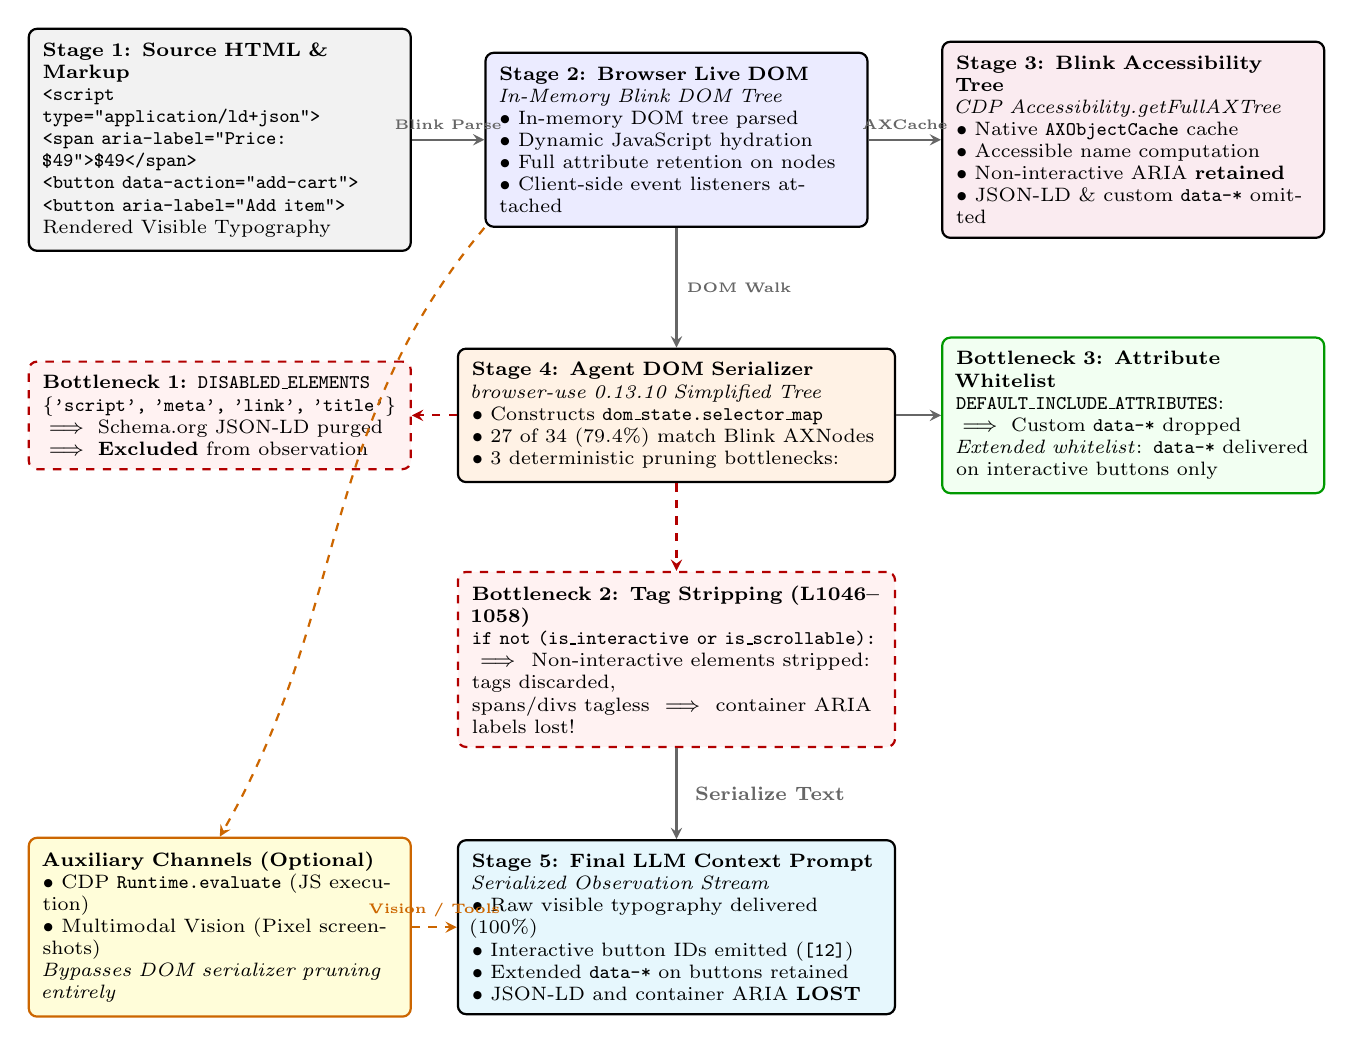
\begin{tikzpicture}[
    box/.style={draw, rounded corners=3pt, thick, align=left, fill=blue!5, font=\scriptsize, inner sep=5pt},
    prunebox/.style={draw=red!70!black, dashed, rounded corners=3pt, thick, align=left, fill=red!5, font=\scriptsize, inner sep=5pt},
    survivebox/.style={draw=green!60!black, rounded corners=3pt, thick, align=left, fill=green!5, font=\scriptsize, inner sep=5pt},
    arrow/.style={->, >=stealth, thick, color=gray!80!black},
    prunearrow/.style={->, >=stealth, dashed, thick, color=red!70!black}
]

% ── Tier 1: Browser Runtime & Representations (Stages 1, 2, 3) ────────────────
\node[box, fill=gray!10, text width=4.5cm] (s1) at (0, 0) {
\textbf{Stage 1: Source HTML \& Markup}\\
\texttt{<script type="application/ld+json">}\\
\texttt{<span aria-label="Price: \$49">\$49</span>}\\
\texttt{<button data-action="add-cart">}\\
\texttt{<button aria-label="Add item">}\\
Rendered Visible Typography
};

\node[box, fill=blue!8, text width=4.5cm] (s2) at (5.8, 0) {
\textbf{Stage 2: Browser Live DOM}\\
\textit{In-Memory Blink DOM Tree}\\
$\bullet$ In-memory DOM tree parsed\\
$\bullet$ Dynamic JavaScript hydration\\
$\bullet$ Full attribute retention on nodes\\
$\bullet$ Client-side event listeners attached
};

\node[box, fill=purple!8, text width=4.5cm] (s3) at (11.6, 0) {
\textbf{Stage 3: Blink Accessibility Tree}\\
\textit{CDP Accessibility.getFullAXTree}\\
$\bullet$ Native \texttt{AXObjectCache} cache\\
$\bullet$ Accessible name computation\\
$\bullet$ Non-interactive ARIA \textbf{retained}\\
$\bullet$ JSON-LD \& custom \texttt{data-*} omitted
};

% ── Tier 2: Agent Serializer & Pruning Bottlenecks (Stage 4) ──────────────────
\node[prunebox, text width=4.5cm] (b1) at (0, -3.5) {
\textbf{Bottleneck 1: \texttt{DISABLED\_ELEMENTS}}\\
\texttt{\{'script', 'meta', 'link', 'title'\}}\\
$\implies$ Schema.org JSON-LD purged\\
$\implies$ \textbf{Excluded} from observation
};

\node[box, fill=orange!10, text width=5.2cm] (s4) at (5.8, -3.5) {
\textbf{Stage 4: Agent DOM Serializer}\\
\textit{browser-use 0.13.10 Simplified Tree}\\
$\bullet$ Constructs \texttt{dom\_state.selector\_map}\\
$\bullet$ 27 of 34 ($79.4\%$) match Blink AXNodes\\
$\bullet$ 3 deterministic pruning bottlenecks:
};

\node[survivebox, text width=4.5cm] (b3) at (11.6, -3.5) {
\textbf{Bottleneck 3: Attribute Whitelist}\\
\texttt{DEFAULT\_INCLUDE\_ATTRIBUTES}:\\
$\implies$ Custom \texttt{data-*} dropped\\
\textit{Extended whitelist}: \texttt{data-*} delivered\\
on interactive buttons only
};

% ── Tier 3: Bottleneck 2 (Tag Stripping) ──────────────────────────────────────
\node[prunebox, text width=5.2cm] (b2) at (5.8, -6.6) {
\textbf{Bottleneck 2: Tag Stripping (L1046--1058)}\\
\texttt{if not (is\_interactive or is\_scrollable):}\\
$\implies$ Non-interactive elements stripped: tags discarded,\\
spans/divs tagless $\implies$ container ARIA labels lost!
};

% ── Tier 4: Model Observation Context & Auxiliary Channels (Stage 5) ─────────
\node[box, fill=yellow!15, draw=orange!80!black, text width=4.5cm] (aux) at (0, -10.0) {
\textbf{Auxiliary Channels (Optional)}\\
$\bullet$ CDP \texttt{Runtime.evaluate} (JS execution)\\
$\bullet$ Multimodal Vision (Pixel screenshots)\\
\textit{Bypasses DOM serializer pruning entirely}
};

\node[box, fill=cyan!10, text width=5.2cm] (s5) at (5.8, -10.0) {
\textbf{Stage 5: Final LLM Context Prompt}\\
\textit{Serialized Observation Stream}\\
$\bullet$ Raw visible typography delivered ($100\%$)\\
$\bullet$ Interactive button IDs emitted (\texttt{[12]})\\
$\bullet$ Extended \texttt{data-*} on buttons retained\\
$\bullet$ JSON-LD and container ARIA \textbf{LOST}
};

% ── Connective Arrows ─────────────────────────────────────────────────────────
\draw[arrow] (s1) -- node[above, font=\tiny\bfseries] {Blink Parse} (s2);
\draw[arrow] (s2) -- node[above, font=\tiny\bfseries] {AXCache} (s3);
\draw[arrow] (s2) -- node[right, font=\tiny\bfseries] {DOM Walk} (s4);

\draw[prunearrow] (s4) -- (b1);
\draw[arrow] (s4) -- (b3);
\draw[prunearrow] (s4) -- (b2);
\draw[arrow] (b2.south) -- node[right=3pt, font=\scriptsize\bfseries] {Serialize Text} (s5.north);

\draw[arrow, dashed, color=orange!80!black] (s2.south west) to[out=230, in=60] (aux.north);
\draw[arrow, dashed, color=orange!80!black] (aux.east) -- node[above, font=\tiny\bfseries] {Vision / Tools} (s5.west);

\end{tikzpicture}%
}
\caption{End-to-end architecture of the autonomous browser agent observation pipeline (\texttt{browser-use 0.13.10}). Web markup transitions across five discrete representations from source HTML to final LLM prompt. Three deterministic pruning bottlenecks in Stage 4 selectively purge structured Schema.org JSON-LD, strip non-interactive WAI-ARIA annotations, and filter custom developer attributes. Auxiliary channels (CDP JavaScript evaluation or visual screenshots) bypass serializer pruning entirely.}
\label{fig:pipeline_architecture}
\end{figure*}


\section{Empirical Systems Audit: The 5-Stage Observation Pipeline}
\label{sec:audit}

\subsection{The 5 Observation Pipeline Stages}
As illustrated in Figure~\ref{fig:pipeline_architecture}, web information flows through distinct representations:
\begin{enumerate}
    \item \textbf{Stage 1 (Source HTML \& Static Markup):} Raw HTML markup received over HTTP.
    \item \textbf{Stage 2 (Browser Live DOM):} In-memory DOM tree parsed by Blink and augmented by client-side JavaScript.
    \item \textbf{Stage 3 (Browser Accessibility Tree):} Chromium Blink native \texttt{AXObjectCache} queried via CDP \texttt{Accessibility.getFullAXTree}. This operates in parallel with DOM serialization.
    \item \textbf{Stage 4 (Agent DOM Serializer):} The simplified selector map and pruned tree constructed by \texttt{browser-use 0.13.10}.
    \item \textbf{Stage 5 (Final Model Context Prompt):} The stringified observation buffer compiled into the LLM context.
\end{enumerate}

Importantly, Stage 3 is not a sequential intermediary between Stage 2 and Stage 4. In \texttt{browser-use 0.13.10}, the serializer walks the live DOM directly (Stage 2 $\to$ Stage 4). Chromium Blink independently constructs its native Accessibility Tree (Stage 2 $\to$ Stage 3).

\subsection{Multi-Stage Observation Retention Matrix}
We executed our automated verification harness (\texttt{audit\_metadata\_reachability.py}) across benchmark variants and edge-case fixtures (\texttt{fixtures/edge\_cases.html}), intercepting prompt payloads using a local \texttt{MockChatModel}. Table~\ref{tab:reachability} reports deterministic retention status across pipeline stages.

\begin{table*}[t]
\centering
\small
\setlength{\tabcolsep}{4pt}
\caption{Multi-stage observation retention matrix across semantic metadata channels in \texttt{browser-use 0.13.10}.}
\label{tab:reachability}
\begin{tabularx}{\textwidth}{>{\raggedright\arraybackslash}p{3.0cm} *{5}{>{\centering\arraybackslash}p{1.35cm}} >{\raggedright\arraybackslash}X}
\toprule
\textbf{Metadata Channel} & \shortstack{\textbf{Stage 1} \\ \scriptsize(HTML)} & \shortstack{\textbf{Stage 2} \\ \scriptsize(Live DOM)} & \shortstack{\textbf{Stage 3} \\ \scriptsize(AXTree)} & \shortstack{\textbf{Stage 4} \\ \scriptsize(Serializer)} & \shortstack{\textbf{Stage 5} \\ \scriptsize(Prompt)} & \textbf{Architectural Filtering Mechanism} \\
\midrule
Schema.org JSON-LD       & Retained & Retained & Dropped  & Dropped  & Dropped  & Blacklisted via \texttt{DISABLED\_ELEMENTS} (L18) \\
Button WAI-ARIA          & Retained & Retained & Retained & Retained & Retained & Whitelisted on interactive elements \\
Non-Interactive ARIA     & Retained & Retained & Retained & Dropped  & Dropped  & Non-interactive tags stripped (L1046) \\
Custom \texttt{data-*} (Default)  & Retained & Retained & Dropped  & Dropped  & Dropped  & Omitted from default attribute whitelist \\
Custom \texttt{data-*} (Extended) & Retained & Retained & Dropped  & Retained & Retained & Delivered on buttons under extended whitelist \\
Temporal \texttt{<meta>} & Retained & Retained & Dropped  & Dropped  & Dropped  & Blacklisted via \texttt{DISABLED\_ELEMENTS} (L18) \\
Temporal \texttt{<time>} & Retained & Retained & Retained & Stripped & Retained & Tag stripped; inner text emitted \\
\bottomrule
\end{tabularx}
\end{table*}

\subsection{Node-Level Correspondence: Chromium AXTree vs. Selector Map}
To evaluate structural alignment between Chromium's native accessibility tree and the agent's observation tree, we implemented \texttt{compare\_accessibility\_tree.py}:
\begin{itemize}
    \item CDP \texttt{Accessibility.getFullAXTree} extracts Blink's unique \texttt{backendDOMNodeId} for accessibility nodes.
    \item In \texttt{browser-use 0.13.10}, \texttt{summary.dom\_state.selector\_map} indexes interactive elements containing the matching Blink \texttt{backend\_node\_id}.
\end{itemize}

\textbf{Empirical Findings on Route \texttt{\#home}:}
Across 336 Chromium AXNodes constructed across the page (256 possessing a discrete \texttt{backendDOMNodeId}), \texttt{browser-use 0.13.10} registered 34 elements in its interactive selector map. Exactly \textbf{27 of 34 elements ($79.4\%$)} matched 1-to-1 to a corresponding Blink AXNode.

\textbf{Forensic Evidence for the 7 Unmatched Elements:}
Detailed node-by-node extraction reveals that all 7 unmatched elements are stock-status badge spans across the first 7 product cards:
\begin{lstlisting}[language=HTML]
<span class="product-stock in-stock">In Stock</span>
\end{lstlisting}
These 7 elements were assigned selector indices 69, 84, 99, 114, 129, 144, and 159. Tracing their inclusion through the source code reveals that they were flagged interactive by \texttt{ClickableElementDetector.is\_interactive} (\texttt{clickable\_elements.py:228--240}). This heuristic classifies any element as an interactive icon if it possesses a \texttt{class} attribute and its layout dimensions satisfy $10 \le \text{width} \le 50$ and $10 \le \text{height} \le 50$. In our benchmark styling, the rendered bounding box for each ``In Stock'' badge is exactly $\mathbf{48.625\text{px} \times 15.0\text{px}}$, which falls within the icon heuristic window. In contrast, the 8th product card's badge (``Out of Stock'') rendered at $\mathbf{74.766\text{px} \times 15.0\text{px}}$, exceeding the 50px threshold; consequently, it was correctly classified as non-interactive. Meanwhile, Chromium Blink's native \texttt{AXObjectCache} treats static inline spans as non-interactive text, flattening them into parent card text runs with \texttt{ignored: true} and omitting discrete \texttt{backendDOMNodeId} accessibility nodes.

\textbf{Denominator Legitimacy and Estimand Analysis:}
Whether all 34 elements legitimately belong in the denominator depends on the intended estimand:
\begin{itemize}
    \item \textbf{Framework Operational Perspective ($n=34$):} From the perspective of evaluating \texttt{browser-use}'s observation space, all 34 elements legitimately belong in the denominator. The framework assigns every one of them a selector index and emits them to the language model as actionable, clickable elements. Under this operational census, correspondence is $27/34 = 79.41\%$.
    \item \textbf{Ground-Truth Semantic Interactivity Perspective ($n=27$):} From a web accessibility and semantics perspective, the 7 in-stock badges are false positives generated by heuristic size thresholds. The page contains exactly 27 genuine interactive controls: 9 anchor links, 16 buttons, 1 text input, and 1 search form. Exactly \textbf{27 of 27 ($100.0\%$)} of these true interactive controls match Chromium's native AXTree.
\end{itemize}
Reporting $27/34$ highlights an architectural gap: heuristic DOM pruning can introduce non-interactive false positives into the agent's action space that native browser accessibility engines reject. We report the descriptive census ($27/34 = 79.4\%$) as primary; the Wilson 95\% confidence interval ($[63.2\%, 89.7\%]$) applies only under a superpopulation model generalizing across similar e-commerce layouts.

\subsection{Structural Divergence Between DOM Serialization and Native Accessibility Trees}
Our comparative analysis reveals bidirectional divergence between native accessibility trees and serialized DOM observations:
\begin{itemize}
    \item \textbf{Non-Interactive ARIA Semantics:} Retained by Chromium Blink's AXTree, but stripped by \texttt{browser-use 0.13.10}. In our stimulus markup (\texttt{variants/v2-aria/index.html}), we examine two distinct patterns:
    \begin{enumerate}
        \item Price Span: \texttt{<span class="product-price" aria-label="Price: \$49.99">\$49.99</span>}. Here, the element lacks an explicit ARIA role. Under W3C WAI-ARIA 1.2~\cite{wai_aria12} \S5.2.7 and the Accessible Name and Description Computation (AccName 1.1) specification~\cite{accname11}, elements with \texttt{role="generic"} prohibit author-supplied naming; standard screen readers ignore \texttt{aria-label} on generic spans. Nonetheless, Chromium Blink's internal \texttt{AXObjectCache} constructs an accessibility node with computed name \texttt{"Price: \$49.99"}. In contrast, \texttt{browser-use 0.13.10} strips the tag entirely at line 1046, delivering only the text \texttt{"\$49.99"}.
        \item Rating Span: \texttt{<span class="product-rating" role="img" aria-label="Rating: 4.5 out of 5 stars">...</span>}. Here, the explicit \texttt{role="img"} is a valid naming container under ARIA 1.2. Blink retains the accessible name, but \texttt{browser-use} strips the element because it is non-interactive.
    \end{enumerate}
    \item \textbf{Custom Developer \texttt{data-*} Attributes:} Completely absent from Blink's accessibility tree (custom attributes have no accessibility semantics), but deliverable to the agent on interactive elements when \texttt{include\_attributes} is extended.
\end{itemize}

\section{Methodological Analysis and Experimental Confounds}
\label{sec:methodology}

\subsection{The Action-Label Co-Location Confound}
When ARIA markup does reach the prompt (on interactive \texttt{<button>} elements), augmenting button labels from generic text (e.g., \texttt{"Add to Cart"}) to entity-specific ARIA labels (e.g., \texttt{aria-label="Add SoundFlow Air 3 to cart"}) introduces an acute experimental confound:
\begin{itemize}
    \item In unaugmented baseline (\textsc{ABS}): The agent observes:
    \begin{quote}
    \texttt{SoundFlow Air 3} \\
    \texttt{\$49.99} \\
    \texttt{[12] <button>Add to Cart</button>}
    \end{quote}
    To select the correct product, the agent must perform spatial or structural reference resolution, associating the preceding typography with button \texttt{[12]}.
    \item In entity-augmented ARIA (\textsc{ARIA}): The agent observes:
    \begin{quote}
    \texttt{[12] <button aria-label="Add SoundFlow Air 3 to cart">Add to Cart</button>}
    \end{quote}
    The target product name is now co-located directly inside the clickable element's attributes.
\end{itemize}
We evaluate generic versus entity-specific ARIA labels as distinct conceptual factors. Entity-specific labels can provide genuine disambiguation benefits in dense interfaces, resolving reference ambiguity. However, in experimental ablation studies intended to evaluate the utility of semantic accessibility channels, injecting entity identifiers directly into button labels confounds the manipulation: it replaces multi-node spatial and semantic reasoning with trivial string matching between the task instruction and the interactive element's accessible name.

\subsection{Hardened State-Asserted Verifiers}
In empirical agent benchmarking, relying on self-reported agent text (e.g., ``I have added the product to the cart'') introduces severe measurement error. In our testing harness, all task completions are verified exclusively through deterministic queries against application state:
\begin{itemize}
    \item Direct inspection of backend SQLite database state (e.g., verifying order rows).
    \item Inspection of browser client-side storage (\texttt{localStorage.cartState}).
    \item CDP DOM node attribute verification (e.g., verifying active cart item count attributes).
\end{itemize}

\subsection{Exploratory Cloud Pilot: The Ceiling Effect}
We executed an exploratory cloud pilot across 41 completed trials using Gemini 2.5 Flash Lite via Google AI Studio (`google-genai 1.55.0`) across three experimental arms (13 ABS, 13 ARIA, 15 DATA-CFG) on simple e-commerce tasks. All 41 completed runs achieved task success ($100.0\%$, Wilson 95\% CI: $[91.4\%, 100.0\%]$; ABS: $13/13$ $[77.2\%, 100.0\%]$, ARIA: $13/13$ $[77.2\%, 100.0\%]$, DATA-CFG: $15/15$ $[79.6\%, 100.0\%]$). The observed pairwise risk differences are identically zero ($\hat{\theta} = 0.0$, Newcombe 95\% CI: $[-0.228, +0.228]$). In denominator accounting, 44 total execution attempts were recorded; 3 attempts in Run 26 encountered transient upstream \texttt{503 UNAVAILABLE} network errors and were successfully retried on attempt 4 under the framework's retry policy without data corruption.

Critically, this $100\%$ completion rate represents an acute \textbf{task-battery ceiling effect}: on simple single-product addition and linear form completion tasks, visible typography alone was completely sufficient for task success. Because sample variance was identically zero across all arms, this pilot demonstrates the operational execution stability of the harness, but it \textbf{does not demonstrate behavioral equivalence or treatment efficacy} between metadata formats.

\section{Statistical Power Boundaries and Equivalence Analysis}
\label{sec:power}

\subsection{Task-Stratified CMH and Newcombe Hybrid Score Intervals}
To analyze multi-arm agent experiments without assuming normal approximations near probability boundaries, we implemented exact statistical estimators in pure Python:
\begin{itemize}
    \item \textbf{Cochran--Mantel--Haenszel (CMH) Test:} Tests conditional independence across task strata $k=1, \dots, K$. Audited against the Agresti (2002)~\cite{agresti2002categorical} multicenter clinical benchmark ($K=8$), our implementation yields $\chi^2 = 6.3841, p = 0.01151$, matching published figures to 4 decimal places.
    \item \textbf{Newcombe Hybrid Score Interval (Method 10):} Constructs closed-form risk difference intervals by combining Wilson bounds. Audited against Newcombe (1998)~\cite{newcombe1998interval} ($56/70$ vs. $38/80$), our implementation yields $\hat{\theta} = 0.3250$, 95\% CI: $[+0.1764, +0.4578]$, matching published benchmarks exactly.
\end{itemize}

\textbf{Multiple Comparisons Adjustment:} To control family-wise error rates, Bonferroni correction must distinguish comparison families:
\begin{itemize}
    \item In a 3-arm design (ABS, ARIA, DATA-CFG), there are $\binom{3}{2} = 3$ pairwise comparisons, setting nominal significance to $\alpha = 0.05 / 3 \approx 0.0167$.
    \item When evaluating unpooled exploratory sensitivity contrasts across 5 individual tasks, significance is set to $\alpha = 0.05 / 5 = 0.0100$.
\end{itemize}

\subsection{Monte Carlo Power Simulations}
Using a Randomized Complete Block Design (RCBD) across 5 tasks with task-level variance $\sigma^2 = 0.09$ (logit scale), we executed 10,000-trial Monte Carlo power simulations (random seed 42) in `power\_analysis.py` ($n=20$ per arm, $\alpha = 0.0167$):
\begin{itemize}
    \item Large Disparity ($\Delta = 0.70$, $p_0=0.85 \to p_1=0.15$): Power $= 98.6\% \pm 0.3\%$.
    \item Moderate Effect ($\Delta = 0.35$, $p_0=0.80 \to p_1=0.45$): Power $= 49.6\% \pm 1.1\%$.
    \item Small Effect ($\Delta = 0.20$, $p_0=0.80 \to p_1=0.60$): Power $= \mathbf{10.8\% \pm 0.6\%}$.
\end{itemize}
These effect sizes serve as illustrative sensitivity scenarios: at small sample sizes ($n=20$), power to detect a realistic 20-percentage-point difference is only $10.8\%$. Over $89\%$ of such trials will yield a false negative ($p > 0.05$).

\subsection{Sample Size Requirements for TOST Equivalence}
\label{sec:tost}
To demonstrate equivalence between formats within margin $(-\delta_{\text{equiv}}, +\delta_{\text{equiv}})$, researchers must apply the Two One-Sided Tests (TOST) procedure~\cite{schuirmann1987comparison}:
\begin{equation}
n = \left(\frac{(z_{1-\alpha} + z_{(1+\text{power})/2}) \cdot \sqrt{2 \cdot p \cdot (1 - p)}}{\delta_{\text{equiv}}}\right)^2
\end{equation}
where $\text{power} = 1 - \beta$. Under standard equivalence approximations, setting $z_{(1+\text{power})/2} = z_{1 - \beta/2}$ provides a conservative bound ensuring that each one-sided test simultaneously achieves the nominal power. For $\alpha = 0.05$ (one-sided) and $80\%$ power ($1-\beta = 0.80 \implies z_{0.90} = 1.28155$), the combined critical factor is $z_{\text{crit}} = 1.64485 + 1.28155 = 2.92640$. For an illustrative equivalence margin of $\delta_{\text{equiv}} = \pm 0.10$ ($\pm 10$ percentage points):
\begin{itemize}
    \item At $p = 0.70$: Establishing equivalence within $\pm 0.10$ requires $n = 359.8 \approx 360$ trials per arm ($N = 1,080$ for 3 arms, or $N = 1,440$ across 4 arms).
    \item At $p = 0.50$ (maximum variance): Required sample size rises to $n = 428.3 \approx 429$ per arm ($N = 1,287$ for 3 arms).
    \item Clustered Design Effect: If repeated trials within tasks induce clustering ($\rho = 0.10, m = 4 \implies \text{DEFF} = 1 + (m-1)\rho = 1.30$), required sample size increases to $n = 360 \times 1.30 \approx 468$ per arm ($N = 1,404$ for 3 arms).
\end{itemize}
\textbf{Methodological Limitations of the Sizing Model:} We emphasize that an equivalence margin of $\pm 0.10$ is illustrative; it is not an empirically established web-usability tolerance standard. In production settings, smaller degradations may be intolerable, which would dramatically inflate required sample sizes ($n \approx 1,440$/arm for $\delta = \pm 0.05$). Furthermore, the cluster adjustment assumes a constant cluster size $m=4$ and exchangeable intracluster correlation $\rho = 0.10$; in heterogeneous task batteries where correlations vary widely across tasks, cluster-robust generalized estimating equations (GEE) should be employed. Claiming equivalence from small-sample non-significant results ($n=13$ to $20$) constitutes \textbf{The Equivalence Fallacy}.

\section{Discussion: Architectural Trade-Offs and Implications}
\label{sec:discussion}

\subsection{Benefits and Risks of Observation Pruning}
Our findings highlight the fundamental systems tension in browser-agent observation design:
\begin{itemize}
    \item \textbf{Pruning Benefits:} Raw web pages frequently exceed 20,000 DOM nodes and 100,000 tokens. Heuristic pruning dramatically compresses the input context, reduces inference cost, prevents context window exhaustion, and removes noisy subtree boilerplate. Furthermore, stripping non-rendered \texttt{<script>} and \texttt{<style>} tags inadvertently filters out hidden script-embedded text.
    \item \textbf{Pruning Risks:} Overly aggressive pruning discards structured semantic metadata (Schema.org JSON-LD, container ARIA labels, custom attributes) that web authors specifically provide to clarify page meaning. When tags are stripped, semantic relationships between containers and interactive children are lost.
\end{itemize}

\subsection{Implications for Web Standards and Out-of-Band Interfaces}
Proposals to enrich human accessibility trees (WAI-ARIA) specifically for AI scrapers face dual obstacles: first, client-side serializers often strip non-interactive ARIA annotations; second, overloading ARIA with redundant machine metadata risks degrading accessibility tree navigation for human screen-reader users. Consequently, emerging out-of-band protocols---such as \texttt{llms.txt}~\cite{llmstxt2024} and the Model Context Protocol (MCP)~\cite{mcp2024}---offer a cleaner separation of concerns by delivering machine-readable context directly to agents without relying on DOM serialization heuristics.

\section{Limitations}
\label{sec:limitations}

We explicitly identify several key limitations:
\begin{enumerate}
    \item \textbf{Single-Framework Scope:} All AST audits and serialization measurements were conducted on \texttt{browser-use 0.13.10}. Other frameworks (e.g., BrowserGym, Stagehand, Skyvern, Crawl4AI) employ different observation pipelines, accessibility snapshots, or raw HTML distillation heuristics.
    \item \textbf{Observation Modality:} Audits were performed within a text-only observation space (\texttt{use\_vision=False}). Multimodal agents utilizing screenshot inputs can perceive rendered typography and visual styling directly, bypassing DOM serializer pruning.
    \item \textbf{Synthetic Evaluation Environment:} Measurements utilized a controlled e-commerce benchmark environment (\texttt{variants/v0}--\texttt{v3}). While this isolates markup channels from visual occlusions, real-world websites feature dynamic scripts and layout variations not captured in synthetic fixtures.
    \item \textbf{Ceiling Effect and Unexecuted Behavioral Trials:} The 41-trial cloud pilot exhibited a ceiling effect ($100\%$ success across all arms). Demonstrating whether metadata channel reachability translates into statistically significant behavioral differences requires a future channel-isolation experiment (specified in our repository protocol, requiring $N \ge 1,080$ trials for equivalence).
    \item \textbf{Finite Census Scope:} The node correspondence comparison was evaluated on route \texttt{\#home} ($n=34$ interactive elements), producing a finite descriptive census rather than a broad multi-site sample.
\end{enumerate}

\section{Conclusion}
\label{sec:conclusion}

This paper presents an empirical systems audit of the DOM serialization gap in autonomous browser agents, establishing that default observation pipelines in \texttt{browser-use 0.13.10} deterministically prune structured metadata (Schema.org JSON-LD and custom developer attributes) and strip non-interactive container ARIA annotations prior to model prompt construction. We have documented structural divergence between native browser accessibility trees and DOM serializers, formalized the Action-Label Co-Location Confound, and established analytical sample-size boundaries for web agent benchmarks. By providing an entirely reproducible offline verification suite, this work establishes essential systems baselines for future web agent architecture and evaluation.

\bibliographystyle{plain}
\bibliography{references}

\clearpage
\appendix

\section{Offline Statistical Pipeline Verification Benchmark}
\label{app:benchmark}

\textbf{Synthetic Software Benchmark Disclaimer:} The metrics in Tables~\ref{tab:synth1} and~\ref{tab:synth2} are generated from a mock/synthetic benchmark dataset (\texttt{test\_scratch\_synthetic\_data/dataset\_1\_valid\_complete.csv}) to verify that \texttt{analyze\_v3\_results.py} executes without numerical or serialization errors. \textbf{They do not represent real agent task performance.}

\begin{table*}[t]
\centering
\small
\caption{Synthetic software pipeline output: Unpooled sensitivity contrasts across baseline arms (Tasks T1--T5, Bonferroni $\alpha = 0.0100$ for 5 contrasts). Pooling baseline conditions is rejected to prevent the Equivalence Fallacy in the absence of a formal TOST margin.}
\label{tab:synth1}
\begin{tabular*}{\textwidth}{@{\extracolsep{\fill}}lcccccc@{}}
\toprule
\textbf{Contrast ID} & \shortstack{\textbf{Treatment} \\ \scriptsize($n/N$, \%)} & \shortstack{\textbf{Reference} \\ \scriptsize($n/N$, \%)} & \shortstack{\textbf{Risk Diff} \\ \scriptsize($\hat{\theta}$)} & \textbf{Newcombe 95\% CI} & \shortstack{\textbf{CMH} \\ \scriptsize($\chi^2$)} & \shortstack{\textbf{Adjusted} \\ \scriptsize($p$-value)} \\
\midrule
\textsc{ARIA vs BASELINE (ABS)}          & 14 / 20 (70.0\%) & 13 / 20 (65.0\%) & \textbf{+0.0500} & [-0.2312, +0.3168] & 0.000 & 1.0000 \\
\textsc{ARIA vs BASELINE\_REP (VIS)}      & 14 / 20 (70.0\%) & 12 / 20 (60.0\%) & \textbf{+0.1000} & [-0.1901, +0.3644] & 0.178 & 1.0000 \\
\textsc{DATA-CFG vs BASELINE (ABS)}      & 17 / 20 (85.0\%) & 13 / 20 (65.0\%) & \textbf{+0.2000} & [-0.0754, +0.4320] & 1.488 & 1.0000 \\
\textsc{DATA-CFG vs BASELINE\_REP (VIS)}  & 17 / 20 (85.0\%) & 12 / 20 (60.0\%) & \textbf{+0.2500} & [-0.0267, +0.4795] & 2.404 & 0.6050 \\
\textsc{ARIA vs DATA-CFG}               & 14 / 20 (70.0\%) & 17 / 20 (85.0\%) & \textbf{-0.1500} & [-0.3751, +0.0906] & 0.683 & 1.0000 \\
\bottomrule
\end{tabular*}
\end{table*}

\begin{table*}[t]
\centering
\small
\setlength{\tabcolsep}{5pt}
\caption{Baseline stability and quality control check on synthetic benchmark data.}
\label{tab:synth2}
\begin{tabularx}{\textwidth}{>{\raggedright\arraybackslash}p{3.4cm} >{\centering\arraybackslash}p{2.0cm} >{\centering\arraybackslash}p{2.0cm} >{\centering\arraybackslash}p{3.4cm} >{\centering\arraybackslash}X}
\toprule
\textbf{Condition} & \shortstack{\textbf{Success} \\ \scriptsize($n/N$)} & \shortstack{\textbf{Success Rate} \\ \scriptsize(\%)} & \shortstack{\textbf{Baseline Difference} \\ \scriptsize($\hat{\theta}$ and 95\% CI)} & \shortstack{\textbf{Fisher's Exact Test} \\ \scriptsize($p$-value)} \\
\midrule
\textsc{BASELINE (ABS)}     & 13 / 20 & 65.0\% & \multirow{2}{*}{\shortstack{$+0.0500$ \\ \scriptsize 95\% CI: $[-0.2312, +0.3168]$}} & \multirow{2}{*}{\shortstack{$p = 1.0000$ \\ \scriptsize (two-tailed, unadjusted)}} \\
\textsc{BASELINE\_REP (VIS)} & 12 / 20 & 60.0\% & & \\
\midrule
\multicolumn{5}{p{\dimexpr\textwidth-2\tabcolsep\relax}}{\textbf{Methodological Decision on Baseline Pooling:} A two-tailed Fisher's exact test fails to reject the null hypothesis of equal baseline performance ($p = 1.0000 \ge 0.05$). Under statistical equivalence principles, failure to detect a difference cannot be equated with evidence of equivalence (\textit{The Equivalence Fallacy}). In the absence of an \textit{a priori} prespecified Two One-Sided Tests (TOST) equivalence margin ($\delta_{\text{equiv}}$), pooling the two baseline conditions is unjustified. Consequently, baseline conditions are evaluated and reported unpooled in all primary sensitivity contrasts (Table~\ref{tab:synth1}).} \\
\bottomrule
\end{tabularx}
\end{table*}

\clearpage
\section{Exploratory Local Hardware Diagnostics \& Cancellation Telemetry}
\label{app:local_diagnostics}

To inspect execution dynamics on constrained local hardware, we conducted five exploratory diagnostic runs on local quantized \texttt{qwen2.5:7b-instruct-q4\_K\_M} via Ollama on hybrid CPU/GPU hardware (AMD Ryzen 5 5600H, 16 GB DDR4 RAM, NVIDIA GeForce RTX 3050 Laptop GPU with 4 GB VRAM). Table~\ref{tab:qwen_runs} reports the telemetry from \texttt{results/local\_pilot\_raw\_logs.json}.

\begin{table*}[t]
\centering
\small
\setlength{\tabcolsep}{4pt}
\caption{Exploratory diagnostic runs on local \texttt{qwen2.5:7b-instruct-q4\_K\_M} (Task T2).}
\label{tab:qwen_runs}
\begin{tabularx}{\textwidth}{>{\raggedright\arraybackslash}p{2.6cm} >{\raggedright\arraybackslash}p{1.8cm} >{\raggedright\arraybackslash}p{2.1cm} cc >{\centering\arraybackslash}p{2.0cm} >{\raggedright\arraybackslash}X}
\toprule
\textbf{Run ID} & \textbf{Arm} & \textbf{Variant} & \textbf{Duration} & \textbf{Steps} & \shortstack{\textbf{CDP State} \\ \scriptsize(Ground Truth)} & \textbf{Observed Mechanism} \\
\midrule
\texttt{qwen\_diag\_001} & \textsc{DATA-CFG} & \texttt{v3-data-attrs} & 3.34s    & 0 & False      & Pydantic validator exception (\texttt{max\_history\_items} parameter constraint). \\
\texttt{qwen\_diag\_002} & \textsc{DATA-CFG} & \texttt{v3-data-attrs} & 1013.09s & 2 & \textbf{True (1.0)} & Step 2 clicked button; Step 3 blocked until HTTP read timeout due to missing outer watchdog. \\
\texttt{qwen\_diag\_003} & \textsc{DATA-CFG} & \texttt{v3-data-attrs} & 288.61s  & 2 & \textbf{True (1.0)} & Step 1 succeeded (102.9s); Step 2 breached 180s watchdog ceiling. \\
\texttt{qwen\_diag\_004} & \textsc{ABS}      & \texttt{v3-data-attrs} & 185.50s  & 1 & False      & Step 1 watchdog timeout; unhandled cancellation dropped telemetry. \\
\texttt{qwen\_diag\_005} & \textsc{ABS}      & \texttt{v3-data-attrs} & 188.56s  & 1 & False      & Step 1 watchdog timeout; cancellation telemetry safely captured. \\
\bottomrule
\end{tabularx}
\end{table*}

\textbf{Telemetry Analysis and Harness Observations:}
\begin{itemize}
    \item \textbf{Watchdog Ceilings vs. Hardware Latency:} In run 003, with prompt expansion exceeding 3,200 tokens across multi-turn history, prompt ingestion and generation latency combined to exceed the 180-second per-step watchdog, triggering execution termination. Post-hoc verification confirmed that the cart interaction had completed prior to timeout.
    \item \textbf{Cancellation Telemetry Capture:} In Python 3.8+, \texttt{asyncio.CancelledError} inherits from \texttt{BaseException}. In run 004, standard \texttt{except Exception:} handlers failed to catch watchdog cancellations. In run 005, dedicated \texttt{except asyncio.CancelledError:} handling successfully logged the in-flight timeout without corrupting trial records.
\end{itemize}
These five exploratory runs illustrate harness engineering boundaries and watchdog behavior under local execution; they do not represent generalizable findings on model reasoning capabilities.

\clearpage
\section{In-Process Request Metering and Quota Governance Architecture}
\label{app:quota_governance}

During experimental agent evaluation, unexpected multi-turn loops or runaway concurrency can exhaust API rate limits or incur unintended costs. In our testing harness, client-side requests are bounded via a thread-safe, fail-closed quota architecture implemented in \texttt{budget\_controller.py}:
\begin{itemize}
    \item \textbf{Pre-Dispatch Reservation:} A proxy model wrapper (\texttt{BudgetGuardedChatModel}) intercepts every invocation of \texttt{ainvoke()} immediately prior to network transmission. Under a re-entrant thread lock (\texttt{threading.RLock}), it queries \texttt{check\_can\_dispatch\_request()}. If cumulative requests meet or exceed the ceiling (e.g., 600 requests), it raises \texttt{BudgetExceededError}, failing closed.
    \item \textbf{Atomic Reservation Accounting:} Upon clearance, \texttt{record\_request\_pre\_dispatch()} atomically increments the persistent request counter on disk before the network socket opens. Even if the subsequent HTTP request drops or times out, the attempt is accounted for against the ceiling.
    \item \textbf{Post-Dispatch Token Reconciliation:} Following successful completion, \texttt{record\_request\_post\_dispatch()} reconciles prompt and completion token counts using provider-reported usage metadata, updating cost calculations without double-counting the request.
    \item \textbf{Trial Finalization Decoupling:} At trial completion, \texttt{record\_trial\_completion(requests\_already\_recorded=True)} increments trial metrics without re-incrementing the request counter, guaranteeing exact 1-to-1 metering.
\end{itemize}
\textbf{Scope and Operational Boundaries:} This architecture guarantees strict request ceilings within a single Python runtime and concurrency model. It does not provide inter-process synchronization across multiple external script invocations, nor does it replace provider-side billing console caps.

\clearpage
\section{Step-by-Step Offline Reproducibility Instructions}
\label{app:reproduce}

All systems findings and statistical bounds reported in this paper can be reproduced offline on Windows or Linux environments in under two minutes without network access or live API calls:
\begin{enumerate}
    \item \textbf{Full Automated Test Suite (126 Tests):}
    Verify all 126 regression and integration tests across quota controls, verifiers, and pipeline stages ($100\%$ passing in $\sim 15$s):
\begin{lstlisting}
python -m unittest discover -s . -p "test_*.py"
\end{lstlisting}

    \item \textbf{Multi-Channel Reachability Trace (Table~\ref{tab:reachability}):}
    Trace metadata retention across the 5-stage observation pipeline to generate \texttt{serialization\_audit\_metrics.json}:
\begin{lstlisting}
python audit_metadata_reachability.py
\end{lstlisting}

    \item \textbf{Chromium Blink AXTree vs. Serializer Comparison (Section~\ref{sec:audit}):}
    Extract Blink accessibility nodes via CDP and evaluate correspondence against \texttt{browser-use}:
\begin{lstlisting}
python compare_accessibility_tree.py
\end{lstlisting}

    \item \textbf{TOST Power Bounds Reproduction (Section~\ref{sec:tost}):}
    Compute required sample sizes for statistical equivalence testing under varying margins ($N \ge 1,440$ across 4 arms, $n \approx 360$/arm at $p=0.70$, $\delta = \pm 0.10$):
\begin{lstlisting}
python reproduce_power_audit.py
\end{lstlisting}

    \item \textbf{Statistical Engine Clinical Benchmark (Appendix~\ref{app:benchmark}):}
    Validate Newcombe hybrid score CIs, Cochran-Mantel-Haenszel tests, and Fisher's exact tests against clinical reference datasets:
\begin{lstlisting}
python -m unittest test_analyze_v3_results.py
\end{lstlisting}
\end{enumerate}

\end{document}
